\subsection{Host CPU}

Abbildung \ref{fig:arch_02} zeigt die Komponenten welche für Echtzeit-Audio auf der CPU benötigt werden. Audio-Hardware benötigt, einen kontinuierliches genau-getaktetes Datenstrom um es den Digital-Analog-Wandlern bereitzustellen. Dies geschieht durch periodisches Abfragen des Betriebssystems über die Hardware-Interrupts. Die angeforderte Puffergrße kann wenige Abtastwerte beinhalten und die Abfrageintervall weniger als 1 ms. Dies ist abhängig von der benützten Hardware und der Audio-Treiber.

Das Betriebssystem bietet eine Abstraktionsschicht in Form einer API für die Anwendungssoftware. Dies gibt der Anwendungs-Software einer einheitlichen Schnittstelle, unabhängig von der Marke der Audio-Hardware und Treiber.

Das VST-API ist eine weitere Abstraktionsschicht, die weiderum eine einheitliche Schnittstelle für Plugin-Anbieter anbietet, unabhängig von der OS. Aber VST ist nicht die einzige Plugin API. Die JUCE Bibliothek bietet einen eigenen Plugin-API, die einfacher ist und abstrahiert die Unterschiede zwischen verschiedene Plugin-APIs.

Die Datenanabfrage, ausgelöst duch Interrupts von der Audio-Hardware, werden durch das Betriebssystems an die DAW-Anwendung durch Rückruffunktionen weitergeleitet. Das DAW hat zuvor, beim aufstarten, die entsprechende Rückrufffunktionen an das Betriebssystems registriert. Die DAW-Anwendung wiederum lietet die Datenabfrage, ebenfalls duch die vom VST Spzifizierten Rückruffunktionen an alle aktiven Plug-ins weiter.

\begin{figure}[H]
    \centering
    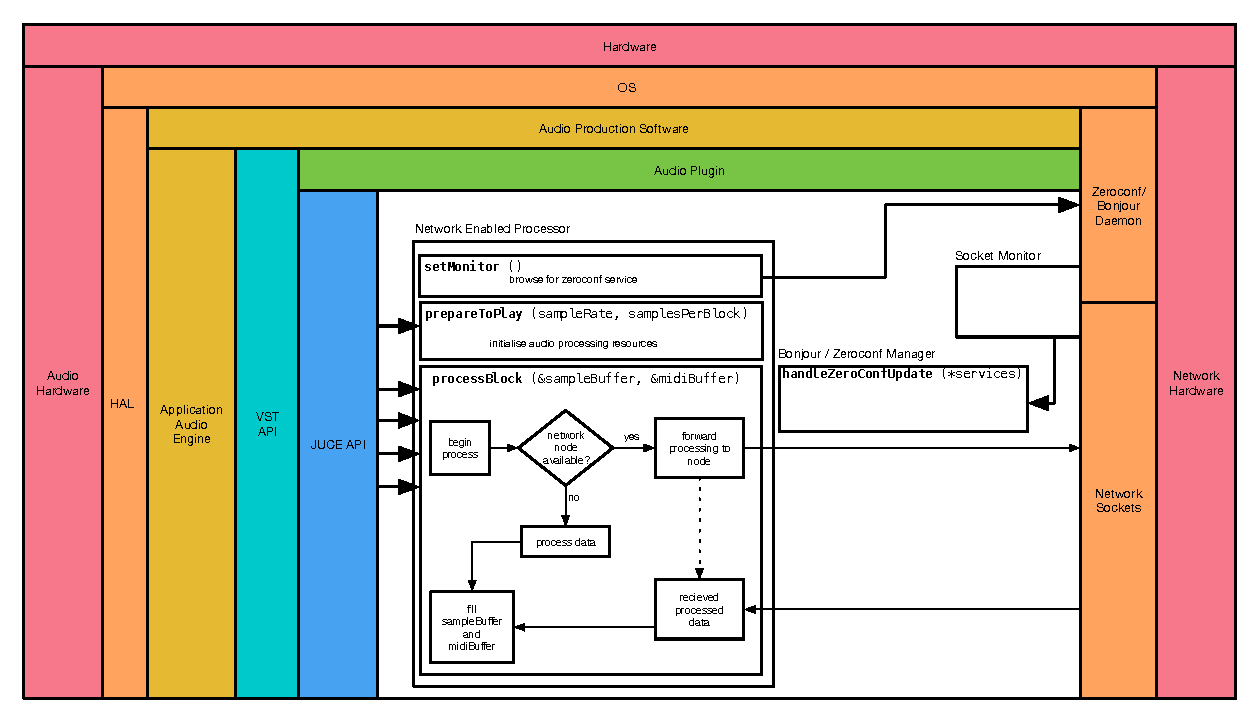
\includegraphics[width=\textwidth]{assets/architecture_02.pdf}
    \caption{Host CPU Überblick}
    \label{fig:arch_02}
\end{figure}

Die für dieses Projekt umgesetztes Audio Plug-in hat mehrere Netzwerkprozessoren aktiviert, in Abbildung \ref{fig:arch_02} wird nur eine dargestellt als Beispiel. Wenn das Plug-in von der Host-Software instanziiert wird, instanziiert es weiderum jeder seiner internen Prozessoren. Die Prozessoren rufen je den Bonjour / Zeroconf-Daemon des Betriebssystems auf, um eine passende im Netzwerk registriertes Rechenknoten zu finden. Der Aufruf übergibt das Daemon eine Socket über eine benachrichtigung zurück schicken kann wenn es einen passendes Service im Netzwerk gefunden hat.

Die Bonjour / Zeroconf-Daemon übergibt dem Audio Plug-in mittels der Socket einer Liste der gefundenen Services. Die Audio Plug-in durchsucht die Liste nach einer freien Rechenkonten. Das ausgewählter Rechenknoten wird in das "activeNode" Variable gespeichert.

Wenn eine Anfrage für Audio-Daten von der DAW-Anwendung an das Plugin übergeben wird, dann wird der "processBlock" Funktion des Plugins aufgerufen. Das Plugin ruft wiederum die "processBlock" Funktionen jedes seiner internen Audio Prozessoren nacheinander. In Abbildung \ref{fig:arch_02} wird dies vereinfacht dargestellt, mit der "processBlock" Funktion von einem einzigen Audio Prozessor. Der "processBlock" Funktion wird einen Referenz auf die aktuelle zu verarbeiten Audiopuffer und MIDI-Puffer übergegeben. Der Audiopuffer enthält die einzelnen Audioabtastungen für jeden Kanal als Float-Werte. Die MIDI-Puffer enthält Performance-Daten wie der Eintrittszeit und Tonhöhe der gespielten Noten.

Innerhalb der "processBlock" Funktion prüft der Prozessor, ob ein Rechenknoten im "activeNode" gespeichert ist. Wenn ja, dann leitet er sofort die MIDI- und Audiodaten sowie die eigene Zustandsdaten an die Rechenknoten und wartet auf die Antwort. Wenn die Antwort eintrifft werden die Daten zurück in die entsprechende Puffer kopiert. Die DAW-Anwendung geht dann weiter die nächsten Plug-ins abfragen, bis die gesamte Verarbeitungskette abgeschlossen ist. Die resultierenden Puffer wird an die Audiohardware über die HAL API geschickt.